% Created: Enze Chen, June 2017

% Chapter 6 of the MSE 142 coursereader. 
% This chapter discusses parabolic potentials and the quantum harmonic oscillator. 
% Students are introduced to operators, and in particular use the ladder operators to solve the Schrodinger equation. 
% A wealth of additional properties are rather lamely appended to the last section.

% Uncomment the following three lines and last line to individually compile this chapter
%\documentclass[12pt, english]{book}
%\usepackage{142crstyle}
%\begin{document}

\chapter{Quantum Harmonic Oscillators} \label{ch:qho}
%{ \doublespacing 
In this chapter, we will consider what happens when a particle is placed in a parabolic potential, which lacks the sharp discontinuities present in previous examples. 
We will see some pretty amazing behavior when we try to solve the \Sch\ equation for this non-constant potential, which will give us a much better understanding of quantization in quantum mechanical systems.


% % % % % % % % % % % % % % % % % % % % % % % % % % % % % % % % % % % % % 
% % % % % % % % % % % % % % % % % % % % % % % % % % % % % % % % % % % % % 
% % % % % % % % % % % % % % % % % % % % % % % % % % % % % % % % % % % % % 
\section{Before you begin}

This chapter builds on the following concepts, some of which we've already discussed in class, others you will likely have encountered elsewhere.
Mastery of these concepts will allow you to get the most out of this chapter.

\begin{itemize}
	\item Simple harmonic oscillators.
	We provide a short review in \autoref{sec:shm}.
	
	\item Complex numbers, especially multiplying complex conjugates.
	
	\item Single-variable integration, which you can review using \href{https://tutorial.math.lamar.edu/Classes/CalcII/IntTechIntro.aspx}{Paul's Online Math Notes}.
\end{itemize}

\begin{tcolorbox}[colframe=PaloAlto, colbacktitle=PaloAlto!20!white, title=Self-check quiz]
	We strongly recommend everyone to take \href{https://forms.gle/GYa2V1pGq7MBqhi99}{the autograded quiz} for this chapter \emph{before} you begin.
	It is anonymous and doesn't affect your grade, but it will give you some feedback and situate you for what's about to come.
\end{tcolorbox}



% % % % % % % % % % % % % % % % % % % % % % % % % % % % % % % % % % % % % 
% % % % % % % % % % % % % % % % % % % % % % % % % % % % % % % % % % % % % 
% % % % % % % % % % % % % % % % % % % % % % % % % % % % % % % % % % % % % 
\section{Parabolic potential}

Consider a one-dimensional quadratic potential energy surface given by $V(x) = \frac{1}{2} kx^2$ which is typically associated with harmonic oscillators. 
Like the simple harmonic oscillator, the \textbf{quantum harmonic oscillator} (QHO) also has an effective spring constant $k$ and an associated angular frequency $\omega$ that is related by $\omega = \sqrt{k/m}$. 
The QHO is a powerful model for things like the forces that hold atoms together in materials and any potential energy surface near a local minimum (\autoref{fig:qpot}).

\begin{figure}[!h]
	\centering
	\subfloat[]{\raisebox{1.7\height}{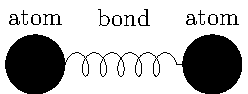
\includegraphics[width=0.25\linewidth]{atoms-spring.pdf}} \label{fig:qho-mod1}} \hspace{4ex}
	\subfloat[]{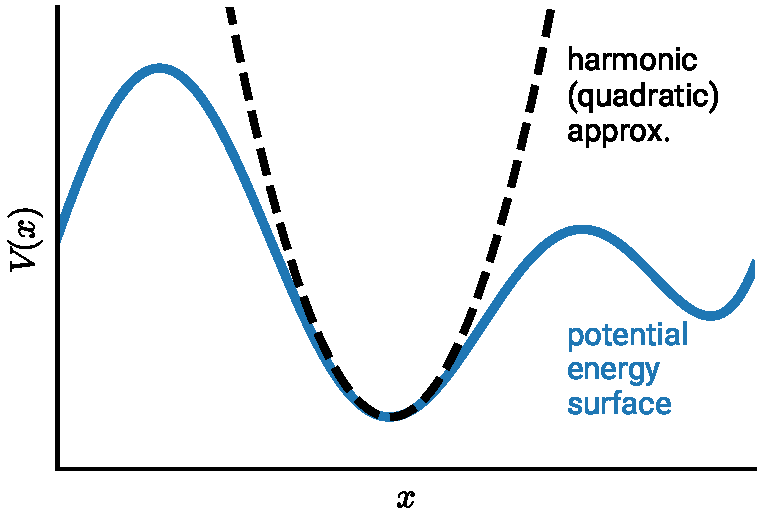
\includegraphics[width=0.43\linewidth]{qpot-min.pdf} \label{fig:qho-mod2}}
	\caption{The quantum harmonic oscillator is particularly powerful at modeling \protect\subref{fig:qho-mod1} the forces that hold atoms together, which are often approximated with springs, and 
	\protect\subref{fig:qho-mod2} the minima of any generic potential surface, which is approximately parabolic when one considers the Taylor series near the minimum.}
	\label{fig:qpot}
\end{figure}



% % % % % % % % % % % % % % % % % % % % % % % % % % % % % % % % % % % % % 
% % % % % % % % % % % % % % % % % % % % % % % % % % % % % % % % % % % % % 
% % % % % % % % % % % % % % % % % % % % % % % % % % % % % % % % % % % % % 
\section{Operators}

In order to work with the QHO, we will have to revisit the concept of \textbf{operators}, which are just special functions that represent physical observables. 
If we represent the quadratic potential energy in terms of angular frequency, i.e. $V(x) = \frac{1}{2} m\omega^2x^2$, we can then represent the Hamiltonian of the particle, which is the sum of the kinetic and potential energies, as

\begin{tcolorbox}[title = Hamiltonian for the QHO] \vspace{-2ex}
	\begin{equation}
	\hat{H} = \frac{\hat{p}^2}{2m} + \frac{1}{2}m\omega^2x^2 \label{eq:ham-qho}
	\end{equation}
\end{tcolorbox}

Notice that in the first term, we used $\hat{p}$ to represent the momentum operator, which is defined as $\hat{p} = -i\hbar\dv{x}$.\footnote{Technically position here is also an operator $\hat{x}$, but it \href{https://physics.stackexchange.com/questions/273272/derivation-of-position-operator-in-qm}{happens to be defined} as $\hat{x} = x$, so we leave off the hat.} 
Now we need to solve the time-independent \Sch\ equation, given by:

\begin{tcolorbox}[title = \Sch\ equation for the QHO] \vspace{-2ex}
	\begin{equation}
		\hat{H}\Psi = -\frac{\hbar^2}{2m}\dv[2]{\Psi}{x} + \frac{1}{2}m\omega^2x^2\Psi = E\Psi \label{eq:se-qho}
	\end{equation}
\end{tcolorbox}

Recall that this form for the operator $\hat{p}$ was motivated by the first wave equation we wrote down, corresponding to the free particle. 
This was an expression of the form $\exp\left(i(kx-\omega t)\right) = \exp \left( \frac{i}{\hbar}(px-Et) \right)$. 
If we act on this wave equation with the operator $\hat{p}$ defined as above, we get the same function back multiplied by $p$:

\begin{align*}
	\hat{p}\exp \left(\frac{i}{\hbar}(px-Et)\right) &= -i\hbar\exp \left(\frac{i}{\hbar}(px-Et)\right) \left(\frac{ip}{\hbar}\right) \\
	&= p\exp \left(\frac{i}{\hbar}(px-Et)\right)
\end{align*}

One can think of this as essentially representative of what it means to make a measurement of the momentum in a quantum mechanical system.



% % % % % % % % % % % % % % % % % % % % % % % % % % % % % % % % % % % % % 
% % % % % % % % % % % % % % % % % % % % % % % % % % % % % % % % % % % % % 
% % % % % % % % % % % % % % % % % % % % % % % % % % % % % % % % % % % % % 
\subsection{Ladder operators}

In order to solve \autoref{eq:se-qho}, we will attempt to \emph{factor} the Hamiltonian given by \autoref{eq:ham-qho}. 
To see the motivation behind this, notice that if the Hamiltonian was given by two real numbers $c^2 + d^2$, we could then factor this expression as 

\begin{equation*}
	c^2 + d^2 = (c + di)(c - di)
\end{equation*}

Following this example, we first reformulate the Hamiltonian so that we can factor it as follows:

\begin{align*}
	\hat{H} &= \frac{\hat{p}^2 }{2m} + \frac{1}{2}m\omega^2\hat{x}^2 \\
	&= \frac{m\omega^2}{2}\left[\hat{x}^2 + \frac{\hat{p}^2}{m^2\omega^2}\right] \\
	&= \frac{m\omega^2}{2}\left[\hat{x} + \frac{i\hat{p}}{m\omega}\right] \left[\hat{x}-\frac{i\hat{p}}{m\omega}\right] \numberthis \label{eq:ham-factored}
\end{align*}

\emph{A word of caution}: Though it may seem logical, we actually hand-waved a lot of the rigor here, because dealing with operators (which are functions) is trickier than dealing with real quantities (i.e., scalars). 
The theory is outside the scope of this course, but we will see shortly how this affects what are normally intuitive results. 

Now, the factored Hamiltonian in \autoref{eq:ham-factored} is suggestive of some form of symmetry, particularly the expressions inside the square brackets. 
We are now going to define two new operators:

\begin{tcolorbox}[title = Ladder operators] \vspace{-2ex}
	\begin{align}
		a &= \sqrt{\frac{m\omega}{2\hbar}}\left(\hat{x} + \frac{i\hat{p}}{m\omega}\right) = \sqrt{\frac{m\omega}{2\hbar}}\left(\hat{x} + \frac{\hbar}{m\omega}\dv{x}\right) \label{eq:annihile} \\
		\ad &= \sqrt{\frac{m\omega}{2\hbar}}\left(\hat{x} - \frac{i\hat{p}}{m\omega}\right) = \sqrt{\frac{m\omega}{2\hbar}}\left(\hat{x} - \frac{\hbar}{m\omega}\dv{x}\right) \label{eq:creation}
	\end{align}
\end{tcolorbox}

The method we are using to solve the \Sch\ equation in this chapter involves these two \textbf{ladder operators} $a$ and $\ad$ (read as: ``a-dagger"), which are known as the \textbf{annihilation}/\textbf{lowering} operator and \textbf{creation}/\textbf{raising} operator respectively (you will soon see why). 
This clever method was developed by Paul Dirac\footnote{Dirac was extremely influential in developing the formalism of quantum theory, introducing this and bra-ket notation which you will see later. He shared the 1933 Nobel Prize in Physics with \Sch. Curiously, Einstein describes that ``[he has] trouble with Dirac. This balancing on the dizzying path between genius and madness is awful.'' (N. Sukumar, \emph{A Matter of Density}, 2012).} and allows us to eventually solve for the energy without directly solving the \Sch\ equation. 
Note that we chose the coefficient of $\sqrt{m\omega/2\hbar}$ largely for the purpose of eliminating constants in the end.


% % % % % % % % % % % % % % % % % % % % % % % % % % % % % % % % % % % % % 
% % % % % % % % % % % % % % % % % % % % % % % % % % % % % % % % % % % % % 
% % % % % % % % % % % % % % % % % % % % % % % % % % % % % % % % % % % % % 
\subsection{Hamiltonian revisited}

We see that the ladder operators are individually defined in terms of the position and momentum operators, so why not try solving for them? 
If we add \autoref{eq:annihile} and \ref{eq:creation}, we get 

\begin{equation*}
	a + \ad = \sqrt{\frac{m\omega}{2\hbar}}2\hat{x}
\end{equation*}

\noindent which allows us to solve for the position operator as

\begin{tcolorbox}[title = Position operator] \vspace{-2ex}
	\begin{equation}
		\hat{x} = \sqrt{\frac{\hbar}{2m\omega}}\left(\ad + a \right) \label{eq:x-op}
	\end{equation}
\end{tcolorbox}

Similarly, we can subtract the two ladder operators to get

\begin{equation*}
	a - \ad = \sqrt{\frac{m\omega}{2\hbar}} \frac{2i\hat{p}}{m\omega}
\end{equation*}

\noindent which gives the momentum operator as 

\begin{tcolorbox}[title = Momentum operator] \vspace{-2ex}
	\begin{equation}
	\hat{p} = i\sqrt{\frac{m\omega\hbar}{2}}\left(\ad - a \right) \label{eq:p-op}
	\end{equation}
\end{tcolorbox}

OK, so why might this be useful? 
Let's rewrite the Hamiltonian in terms of these new operators:

\begin{align*}
	\hat{H} &= \frac{\hat{p}^2}{2m} + \frac{1}{2}m\omega^2\hat{x}^2 \\
	&= -\frac{1}{2m}\frac{m\omega\hbar}{2}\left(\ad - a\right)^2 + \frac{1}{2}m\omega^2 \frac{\hbar}{2m\omega} \left(\ad + a \right)^2 \\
	&= -\frac{\hbar\omega}{4} \left(\left(\ad\right)^2 - \ad a - a\ad + a^2\right) + \frac{\hbar\omega}{4}\left(\left(\ad\right)^2 + \ad a + a\ad + a^2 \right) \\
	\Aboxed{ \hat{H} &= \frac{\hbar\omega}{2} \left( \ad a + a\ad \right)} \numberthis \label{eq:ham-qho2}
\end{align*}

Now, we might be tempted to combine the $\ad a$ term with the $a \ad$ term, but this is one of the tricky aspects of operators: 
\textbf{In general, they do not commute} with each other, so we can't expect them to represent the same quantity when we switch the order. 

Of course, we shouldn't be fazed by this fact and we will try to see if we can find some relationship between the two terms. 
Luckily, in quantum mechanics, there is a quantity called the \textbf{commutator} (adopted from group theory) that precisely indicates to what degree two operators fail to commute. 
Given two operators $A$ and $B$, we define the commutator as

\begin{equation}
	[A,B] = AB - BA \label{eq:comm}
\end{equation}

\noindent which you can see for normal (scalar) variables should be zero.

As a first example, let's consider the commutation relation between $\hat{x}$ and $\hat{p}$, i.e. $[\hat{x}, \hat{p}]$. 
To aid the derivation, we will have both operators act on an arbitrary dummy function $\Psi$ that we will discard in the end.

\begin{align*}
	[\hat{x}, \hat{p}]\Psi &= (\hat{x}\hat{p})\Psi - (\hat{p}\hat{x})\Psi \\
	&= x\left(-i\hbar \dv{x}\Psi \right) + i\hbar \dv{x}(x\Psi) \\
	&= -i\hbar x \dv{x}\Psi + i\hbar x \dv{x}\Psi + i\hbar\Psi \\
	&= i\hbar\Psi 
\end{align*}

From this, one then concludes that 

\begin{tcolorbox}[title = Canonical commutation relation] \vspace{-2ex}
	\begin{equation}
		[\hat{x}, \hat{p}] = i\hbar
	\end{equation}
\end{tcolorbox}

\noindent which is known as the \textbf{canonical commutation relation} because it establishes a fundamental relationship between two conjugate variables, such as $\hat{x}$ and $\hat{p}$, that eventually leads to the uncertainty principle. 

Now what about the commutation relation between $a$ and $\ad$? 
The result actually follows nicely from the canonical commutation relation. 
First, we also show that if two operators can be expressed as $f+g$ and $f-g$, where $f$ and $g$ are arbitrary operators, then their commutation relation can be simplified as follows:

\begin{align*}
	[f+g,f-g] &= (f+g)(f-g) - (f-g)(f+g) \\
	&= f^2 - fg + gf -g^2 - f^2 - fg + gf + g^2 \\
	&= 2(gf - fg) \\
	&= 2[g,f]
\end{align*}

We can apply this result to find that

\begin{align*}
	[a, \ad] &= \frac{m\omega}{2\hbar}\left[\hat{x} + \frac{i\hat{p}}{m\omega}, \hat{x} - \frac{i\hat{p}}{m\omega} \right] \\
	&= \frac{m\omega}{\hbar} \left[ \frac{i\hat{p}}{m\omega}, \hat{x} \right] \\
	&= \frac{i}{\hbar}[\hat{p},\hat{x}] \\
	&= \frac{i}{\hbar}(-i\hbar) = 1
\end{align*}

\begin{tcolorbox}[title = Ladder operators commutation relation] \vspace{-2ex}
	\begin{equation}
		[a,\ad] = a\ad - \ad a = 1  \label{eq:a-comm}
	\end{equation}
\end{tcolorbox}


% % % % % % % % % % % % % % % % % % % % % % % % % % % % % % % % % % % % % 
% % % % % % % % % % % % % % % % % % % % % % % % % % % % % % % % % % % % % 
% % % % % % % % % % % % % % % % % % % % % % % % % % % % % % % % % % % % % 
\section{Solutions of the QHO}

We're almost there! 
Now using this commutation relation, we can rewrite \autoref{eq:ham-qho2} in its standard form. 
In particular, using the fact that $a\ad = 1 + \ad a$, we find that

\begin{tcolorbox}[title = Hamiltonian of the QHO (with ladder operators)] \vspace{-2ex}
	\begin{equation}
	\hat{H} = \hbar\omega \left(\ad a + \frac{1}{2} \right) \label{eq:ham-qho3}
	\end{equation}
\end{tcolorbox}

OK, now let's try to understand why all of the above definitions and mathematics are useful in terms of solving the QHO problem. 
To begin with, let's rewrite the time-independent \Sch\ equation in terms of these new variables. 
We have:

\begin{equation}
	\hbar\omega \left(\ad a + \frac{1}{2} \right)\psi_n = E_n\psi_n \label{eq:sch-qho}
\end{equation}

\noindent where we have introduced a quantum number $n$ as an index for the allowed solutions of this equation, just like we did for the particle in a box. 
Now let's act from the left on \autoref{eq:sch-qho} with the lowering operator $a$, carefully keeping track of the order of the operators since we know they don't commute with each other (but they can commute with scalars, like the energy $E_n$). 
This gives

\begin{align*}
	\hbar\omega \left(\ad a + \frac{1}{2} \right)\psi_n &= E_n\psi_n \\
	\hbar\omega \left(a \ad a + \frac{1}{2} a\right)\psi_n &= E_na\psi_n \\
	\hbar\omega \left(\left(1 + \ad a \right) a + \frac{1}{2} a\right)\psi_n &= E_na\psi_n \\
	\hbar\omega \left(1 + \ad a + \frac{1}{2} \right) a\psi_n &= E_na\psi_n \\
	\Aboxed{\hbar\omega \left(\ad a + \frac{1}{2} \right) (a\psi_n) &= (E_n-\hbar\omega)(a\psi_n)} \numberthis \label{eq:sch-qho2}
\end{align*}

If we look carefully at this equation and compare it to \autoref{eq:sch-qho}, we see that they are the same form! 
This says in particular that if $\psi_n$ is a solution of the QHO with energy $E_n$, then $a\psi_n$ is also a solution, with energy $E_n-\hbar\omega$. 
This is a key result and explains why $a$ is called the lowering operator. 
From a known solution one can essentially generate all other known solutions of lower energy by applying this operator. 
This is quite handy!

So imagine that one starts from some known solution and starts applying this operator, generating lower and lower energy states. 
At some point one must find the ground-state solution. 
But what happens if one then applies the lowering operator to this? 
If this gives some new function, then this can't really have been the ground state! 
We therefore conclude that the ground state wavefunction must satisfy the equation

\begin{equation*}
	a\psi_0 = 0
\end{equation*}

Here you can really see how we have successfully factorized the initial second order differential equation (\autoref{eq:se-qho}) to obtain a solution for the wavefunction. 
In particular, we can use the right hand side of \autoref{eq:annihile} to substitute for the lowering operator $a$ and obtain a first order differential equation:

\begin{equation*}
	\left(x + \frac{\hbar}{m\omega} \dv{x}\right)\psi_0 = 0
\end{equation*}

We can solve this using separation of variables as follows:

\begin{align*}
	\left(x + \frac{\hbar}{m\omega} \dv{x}\right)\psi_0 &= 0 \\
	\frac{\hbar}{m\omega} \dv{\psi_0}{x} &= -x\psi_0 \\
	\frac{1}{\psi_0} \dd{\psi_0} &= -\frac{m\omega}{\hbar}x \dd{x} \\
	\ln (\psi_0) &= -\frac{m\omega}{2\hbar}x^2 \\
	\Aboxed{\psi_0 &= A \exp \left(-\frac{m\omega}{2\hbar}x^2\right)} \numberthis
\end{align*}

We have to normalize the wavefunction the same way we always do, which allows us to solve for $A$ as

\begin{align*}
	\int_{-\infty}^{\infty} \abs{\psi_0}^2 \dd{x} &= 1 \\
	\abs{A}^2 \int_{-\infty}^{\infty} \exp \left(-\frac{m\omega}{\hbar} x^2 \right) \dd{x} &= 1 \\
	\abs{A}^2 \sqrt{\frac{\pi\hbar}{m\omega}} &= 1  \tag{We use $\displaystyle\int_{-\infty}^{\infty}e^{-ax^2} \dd{x} = \sqrt{\frac{\pi}{a}}$}\\
	\Aboxed{A &= \left(\frac{m\omega}{\pi\hbar}\right)^{1/4}} \numberthis
\end{align*}

Combining these two results finally gives us

\begin{tcolorbox}[title = Ground state for the QHO] \vspace{-2ex}
	\begin{equation}
		\psi_0 = \left(\frac{m\omega}{\pi\hbar}\right)^{1/4} \exp \left(-\frac{m\omega}{2\hbar}x^2\right) \label{eq:qho-ground}
	\end{equation}
\end{tcolorbox}

One can easily substitute this back into the \Sch\ equation to verify this indeed solves the differential equation---try it yourself! 
A sketch of this wavefunction has a Gaussian shape within the boundary of the potential with probability maximized at the center of the quadratic potential, analogous to the equilibrium position of the effective mass on a spring (\autoref{fig:qho-ground}). 
The key difference between this state and its classical analogue is that the quantum ground state has non-zero energy.

\begin{figure}[!h]
	\centering
	\includegraphics[width=0.38\linewidth]{qho-ground.pdf}
	\caption{A sketch of the ground state of the particle inside the parabolic potential. 
	The wavefunction has a Gaussian profile within the parabolic potential and it is centered about the minimum.}
	\label{fig:qho-ground}
\end{figure}


% % % % % % % % % % % % % % % % % % % % % % % % % % % % % % % % % % % % % 
% % % % % % % % % % % % % % % % % % % % % % % % % % % % % % % % % % % % % 
% % % % % % % % % % % % % % % % % % % % % % % % % % % % % % % % % % % % % 
\subsection{Zero-point energy}

What is the energy of the particle in this ground state? 
One can substitute \autoref{eq:qho-ground} into the differential equation and solve for $E_0$, or explicitly solve \autoref{eq:sch-qho} when $n = 0$. 
Both approaches work, and we will proceed with the latter approach to obtain

\begin{align*}
	\hbar\omega \left(\ad a + \frac{1}{2} \right)\psi_0 &= E_0\psi_0 \\
	\frac{\hbar\omega}{2}\psi_0 &= E_0\psi_0 \tag{since $a\psi_0=0$}
\end{align*}

\noindent which gives the energy for the ground state as

\begin{tcolorbox}[title = Zero-point energy] \vspace{-2ex}
	\begin{equation}
		E_0 = \frac{\hbar\omega}{2} \label{eq:zpe}
	\end{equation}
\end{tcolorbox}

This ground state energy is commonly referred to as \textbf{zero-point energy}, a concept that we've been alluding to previously. 
The zero-point energy arises due to quantum mechanical fluctuations between energy states that occur even at absolute zero, which explains, for example, why liquid helium does not freeze at standard pressure regardless of temperature.\footnote{Physicists Richard Feynman and John Wheeler have calculated that the zero-point energy in a vacuum the size of a light bulb is enough to boil all the world's oceans. See M. Pilkington, \href{https://www.theguardian.com/education/2003/jul/17/research.highereducation}{\emph{The Guardian}}, 2003.} 
Although it fits the context of the models presented in this course, the physical manifestations of zero-point energy are still poorly understood and are an active area of research.

Now we leave it as an exercise to the reader to show, using a similar procedure as above, that if $\psi_n$ is a solution with energy $E_n$, then $\ad\psi_n$ is also a solution with energy $E_n + \hbar\omega$ and thus $\ad$ behaves as a raising operator. 
Given this, we can now essentially reconstruct all solutions at least in principle by applying the raising operator to the known ground state solution. 
By this procedure, we can write down a clean result for the allowed energy states:

\begin{tcolorbox}[title = Allowed energy states of the QHO] \vspace{-2ex}
	\begin{equation}
		E_n = \hbar\omega\left(n + \frac{1}{2}\right) \label{eq:estates-qho}
	\end{equation}
\end{tcolorbox}

We see that like the particle in a box, the energy states of the QHO are quantized and indexed by the quantum number $n$. 
Where the two differ is that while the energy levels of the particle in a box scale as $n^2$, the energy levels here scale linearly in $n$, which means that these discrete energy levels are equally spaced by $\hbar\omega$. 

Now, you might be asking yourself if this procedure really generates all the possible solutions or just a subset of them. 
The answer is that it really does get them all! 
If there was some other state $\psi_m$ not generated by applying the raising operator successively from the ground state, one could lower this state by successively applying the lowering operator until eventually one arrives at the ground state satisfying $a\psi_0 = 0$. 
But this is just the ground state we've already uniquely identified and indicates that there are no other unique solutions of the \Sch\ equation that we've somehow missed.


% % % % % % % % % % % % % % % % % % % % % % % % % % % % % % % % % % % % % 
% % % % % % % % % % % % % % % % % % % % % % % % % % % % % % % % % % % % % 
% % % % % % % % % % % % % % % % % % % % % % % % % % % % % % % % % % % % %
\section{Additional properties}

\subsection{Bra-ket notation} \label{sec:braket}

We will start by formally introducing some notation to help us from here on out. 
Back in \autoref{ch:intro}, we used $\ket{S}$ as a way to describe quantum states. 
This is standard \textbf{bra-ket notation}, where $\ket{S}$ is called the \textbf{ket} and represents the state of the quantum system, whether it's the momentum, position, or something else. 
Every ket has an associated \emph{dual} or ``left half" called the \textbf{bra}, written as $\bra{S}$. 
Energy states can be expressed as $\ket{\Psi_0}$ or just $\ket{0}$ for short.

As you can probably imagine, the bra and ket can be combined together. 
Specifically, if we have $\bra{\Psi_m}$ and $\ket{\Psi_n}$ representing two quantum states, then this leads to

\begin{tcolorbox}[title = Bra-ket inner product] \vspace{-2ex}
	\begin{equation}
		\braket{\Psi_m}{\Psi_n} = 
		\int_{-\infty}^{\infty} \Psi_m^*\Psi_n \dd{x} \label{eq:bk-int}
	\end{equation}
\end{tcolorbox}

Essentially this notation is representing an \textbf{inner product}, which is a generalization of the dot product that you have seen in previous math classes. 
Indeed, one can think of a bra as a row vector that is multiplying a column vector ket. 
Furthermore, changing a quantum state from a bra to a ket (e.g. $\bra{f} \rightarrow \ket{f}$) is equivalent to taking the \textbf{conjugate transpose}. 
Working with this vector notation, we can also apply operators by multiplying them to the left of a ket, e.g.,

\begin{equation*}
	\hat{H} \ket{\Psi} = E\ket{\Psi} 
\end{equation*}

\noindent where you can treat $\hat{H}$ as an $n\times n$ matrix and $E$ as a constant.


% % % % % % % % % % % % % % % % % % % % % % % % % % % % % % % % % % % % % 
% % % % % % % % % % % % % % % % % % % % % % % % % % % % % % % % % % % % % 
% % % % % % % % % % % % % % % % % % % % % % % % % % % % % % % % % % % % %
\subsection{Expected value}

Since we work with probabilities in quantum mechanics, it is only suitable (and perhaps even delayed at this point) that we cover the concept of \textbf{expectation}, which can be thought of as the \textbf{average} or \textbf{mean} value. 
Given a quantity $x$, we denote the expected value of $x$ by $\expval{x}$. 
In general, the average value of some function of $x$ is given by 

\begin{equation}
	\expval{g(x)} = \sum_{i=1}^{\infty} g(x_i) p(x_i)
\end{equation}

\noindent where $p(x_i)$ is the probability of obtaining $g(x_i)$. 
This is the case for \emph{discrete} variables, such as the expected value of the roll of a die. 
For \emph{continuous} variables, we can't use a single probability for a point (it would be equal to zero), but rather a \textbf{probability density} $\rho(x)$ that can be applied over an interval. 
You're already experienced with probability densities since you've worked with the modulus squared of the wavefunction. 
Now our definition for the expectation of a function of a continuous variable becomes

\begin{equation}
	\expval{f(x)} = \int_{-\infty}^{\infty} f(x) \rho(x) \dd{x}
\end{equation}

When we're working with operators or physical observables, the expectations turn nicely into

\begin{equation}
	\expval{f(x)} = \int_{-\infty}^{\infty} \Psi^* f(x) \Psi \dd{x} = \mel{\Psi}{f}{\Psi} \label{eq:expval}
\end{equation}

Now, a measurement of the energy or momentum must return a real outcome, which means $\expval{f(x)}=\expval{f(x)}^*$. 
This can be rewritten as

\begin{equation*}
	\int_{-\infty}^{\infty} \Psi^* f(x) \Psi \dd{x} = \left( \int_{-\infty}^{\infty} \Psi^* f(x) \Psi \dd{x} \right)^* = \int_{-\infty}^{\infty} \left( f(x) \Psi\right)^* \Psi \dd{x}
\end{equation*}

\noindent or

\begin{equation}
	\braket{\Psi}{f\Psi} = \braket{f\Psi}{\Psi} \label{eq:hermitian}
\end{equation}

This condition defines the operator $f$ as \textbf{Hermitian}, which gives real values for the expectation and has real eigenvalues among its many nice properties. 
As a result, all quantum mechanical operators for physical observables are Hermitian, e.g., momentum, Hamiltonian, position, etc.


% % % % % % % % % % % % % % % % % % % % % % % % % % % % % % % % % % % % % 
% % % % % % % % % % % % % % % % % % % % % % % % % % % % % % % % % % % % % 
% % % % % % % % % % % % % % % % % % % % % % % % % % % % % % % % % % % % %
\subsection{Hermitian conjugates}

We show that $a$ and $\ad$ are \textbf{Hermitian conjugates} (or Hermitian adjoints), which are operators that are related by the following:

\begin{tcolorbox}[title = Hermitian conjugates] \vspace{-2ex}
	\begin{equation}
		\braket{f}{ag} = \braket{\ad f}{g} \label{eq:h-conj}
	\end{equation}
\end{tcolorbox}

\noindent for arbitrary $f$ and $g$. 
If we go back to the integral definition in \autoref{eq:bk-int}, we get that

\begin{equation*}
	\int_{-\infty}^{\infty} f^*ag \dd{x} = \int_{-\infty}^{\infty} (\ad f)^*g \dd{x}
\end{equation*}

\noindent which says that $a$ operating on $g$ must give the same result for the integral as $\ad$ operating on $f$. 
To prove this, we will use the differential form of the operator $a$ and integrate by parts.

\begin{align*}
	\braket{f}{ag} &= \int_{-\infty}^{\infty} f^* \left(x + \frac{\hbar}{m\omega} \dv{x} \right)g \dd{x} \\
	&= \int_{-\infty}^{\infty} f^*xg \dd{x} + \frac{\hbar}{m\omega} \int_{-\infty}^{\infty} f^* \dv{g}{x} \dd{x} \\
	&= \int_{-\infty}^{\infty} f^*xg \dd{x} + \frac{\hbar}{m\omega} \left[ \cancel{f^*g} \bigg|_{-\infty}^{\infty} - \int_{-\infty}^{\infty} \dv{f^*}{x} g \dd{x} \right] \tag{\href{https://tutorial.math.lamar.edu/classes/calcII/IntegrationByParts.aspx}{IBP!}} \\
	&= \int_{-\infty}^{\infty} \left[ \left(x - \frac{\hbar}{m\omega} \dv{x}\right) f \right]^* g \dd{x} \\
	&= \int_{-\infty}^{\infty} \left(\ad f\right)^*g \dd{x} \\
	&= \braket{\ad f}{g} 
\end{align*}

It is also true that

\begin{equation*}
	\braket{f}{\ad g} = \braket{af}{g}
\end{equation*}

We note here that even though the individual ladder operators are Hermitian conjugates, their \emph{product}, which appears in the Hamiltonian, \emph{is} a Hermitian operator.


% % % % % % % % % % % % % % % % % % % % % % % % % % % % % % % % % % % % % 
% % % % % % % % % % % % % % % % % % % % % % % % % % % % % % % % % % % % % 
% % % % % % % % % % % % % % % % % % % % % % % % % % % % % % % % % % % % %
\subsection{Scaling factor}

We already know that the raising and lowering operators generate new solutions of the \Sch\ equation. 
But this is defined only up to a proportionality factor. 
Given a normalized solution like $\psi_0$ found above, how do we find the higher order solutions exactly? 
We could normalize each one by brute force, but there is a nicer way. 
We start by saying that 

\begin{equation*}
	\ad \ket{\psi_n} = c_n \ket{\psi_{n+1}}
\end{equation*}

Next, we can apply the result of \autoref{eq:h-conj} in a clever way and note that

\begin{equation*}
	\braket{\ad \psi_n}{\ad \psi_n} = \braket{a\ad \psi_n}{\psi_n}
\end{equation*}

Then, if we take a closer look at our two expressions for the allowed energy states of the QHO (\autoref{eq:sch-qho} and \ref{eq:estates-qho}), we see that it must be the case that 

\begin{align}
	\ad a \psi_n &= n\psi_n \label{eq:ada-prop} \\
	a \ad \psi_n &= (\ad a + 1)\psi_n = (n+1)\psi_n \label{eq:aad-prop}
\end{align} 

We can combine these results to obtain

\begin{equation*}
	\braket{\ad \psi_n}{\ad \psi_n} = \braket{a\ad \psi_n}{\psi_n} = (n+1) \braket{\psi_n}{\psi_n} = \abs{c_n}^2\braket{\psi_{n+1}}{\psi_{n+1}}
\end{equation*}

Since $\psi_n$ and $\psi_{n+1}$ are normalized, it follows that $\abs{c_n}^2 = n+1$, and we have

\begin{tcolorbox}[title = Raising operator proportionality constant] \vspace{-2ex}
	\begin{equation}
		\ad \psi_n = \sqrt{n+1} \psi_{n+1} \label{eq:ad-prop}
	\end{equation}
\end{tcolorbox}

We will leave it as an exercise to the reader to derive (in essentially the same fashion) the proportionality coefficient for the lowering operator, which is 

\begin{equation}
	a \psi_n = \sqrt{n} \psi_{n-1} \label{eq:a-prop}
\end{equation}


% % % % % % % % % % % % % % % % % % % % % % % % % % % % % % % % % % % % % 
% % % % % % % % % % % % % % % % % % % % % % % % % % % % % % % % % % % % % 
% % % % % % % % % % % % % % % % % % % % % % % % % % % % % % % % % % % % %
\subsection{Orthogonality}
As you may have guessed by now, the stationary state solutions to the QHO are orthogonal,\footnote{In fact they also form an orthonormal basis.} which means that 

\begin{equation}
	\braket{\psi_m}{\psi_n} = \int_{-\infty}^{\infty} \psi_m^*\psi_n \dd{x} = \delta_{mn} \label{eq:ortho_qho}
\end{equation}

We can prove this using \autoref{eq:h-conj} and \ref{eq:ada-prop}. 
First, the second equation gives us

\begin{equation}
	\braket{\psi_m}{\ad a \psi_n} = \braket{\psi_m}{n\psi_n} = n\braket{\psi_m}{\psi_n} \label{eq:qho-orth1}
\end{equation}

However, we can also apply the first equation twice to the left hand side and obtain

\begin{equation}
	\braket{\psi_m}{\ad a \psi_n} = \braket{a \psi_m}{a \psi_n} = \braket{\ad a \psi_m}{\psi_n} = m\braket{\psi_m}{\psi_n} \label{eq:qho-orth2}
\end{equation}

Putting \autoref{eq:qho-orth1} and \ref{eq:qho-orth2} together, one obtains

\begin{equation*}
	(m-n)\braket{\psi_m}{\psi_n} = 0
\end{equation*}

\noindent which shows that if $m \neq n$, then 

\begin{equation*}
	\braket{\psi_m}{\psi_n} = \int_{-\infty}^{\infty} \psi_m^*\psi_n \dd{x} = 0
\end{equation*}

\noindent and the orthogonality condition is satisfied. 


% % % % % % % % % % % % % % % % % % % % % % % % % % % % % % % % % % % % % 
% % % % % % % % % % % % % % % % % % % % % % % % % % % % % % % % % % % % % 
% % % % % % % % % % % % % % % % % % % % % % % % % % % % % % % % % % % % %
\section[Applications]{Applications of the QHO}

By now we've seen just how powerful the QHO model is and how useful some of these properties are. 
The existence of an exact, analytical solution to the QHO makes it a powerful framework for developing more advanced theories to analyze complex quantum mechanical systems. 
We mentioned at the beginning of this chapter how the QHO could be used to model subatomic particles and the forces between atoms, but a proper treatment involves delving a little deeper into \textbf{quantum field theory} (QFT), which is a framework that is partially derived from the concepts presented in this chapter. 
Rather than cramming this rich topic into a section here, we will instead be devoting the entire next chapter to QFT and combining the results from QFT and the QHO to analyze vibrational modes in solids called \textbf{phonons}. 
Stay tuned!

For the time being, however, let's briefly revisit the wavefunction solutions we derived earlier. 
We sidestepped a lot of the ugly algebra by employing the ladder operators method, but I would be doing you a disservice (particularly if you continue to study quantum mechanics in a different field like physics or electrical engineering), if I didn't at least mention the analytic method using \textbf{power series}.\footnote{We will skip all the details here, but there's a thorough derivation in Griffiths, Chapter 2.3.} 
When we work out the math, we arrive at the following expression for the stationary states of the QHO:\footnote{I encourage you to derive another expression for the $n^{\text{th}}$ stationary state using just the ladder operators! \emph{Hint}: The expression is far more concise, albeit recursive.} 

\begin{equation}
	\psi_n(x) = \left(\frac{m\omega}{\pi\hbar}\right)^{1/4} \frac{1}{\sqrt{2^n \cdot n!}} H_n \left(\sqrt{\frac{m\omega}{\hbar}}x\right) \exp \left(-\frac{m\omega x^2}{2\hbar}\right) \label{eq:pow-qho}
\end{equation}

\noindent where $H_n$ are the \textbf{Hermite polynomials}, given explicitly and recursively by

\begin{align*}
	H_n(z) &= (-1)^n e^{z^2} \dv[n]{z} \left( e^{-z^2} \right) \tag{explicit def.} \\
	H_n(z) &= 2zH_{n-1}(z) - 2(n-1)H_{n-2}(z) \tag{recursive def.}
\end{align*}

More concretely, the first few Hermite polynomials are

\begin{align*}
	H_0(z) &= 1 \\
	H_1(z) &= 2z \\
	H_2(z) &= 4z^2-2 \\
	H_3(z) &= 8z^3 - 12z \\
	H_4(z) &= 16z^4 - 48z^2 + 12
\end{align*}

The benefit of this method is that we have a closed-form expression for the wavefunction at any energy level. 
We already saw what the ground state $\psi_0$ looked like, which had maximum amplitude at the center of the quadratic potential, so now we plot $\abs{\psi_{50}}$ in \autoref{fig:qho-50}.

\begin{figure}[!h]
	\centering
	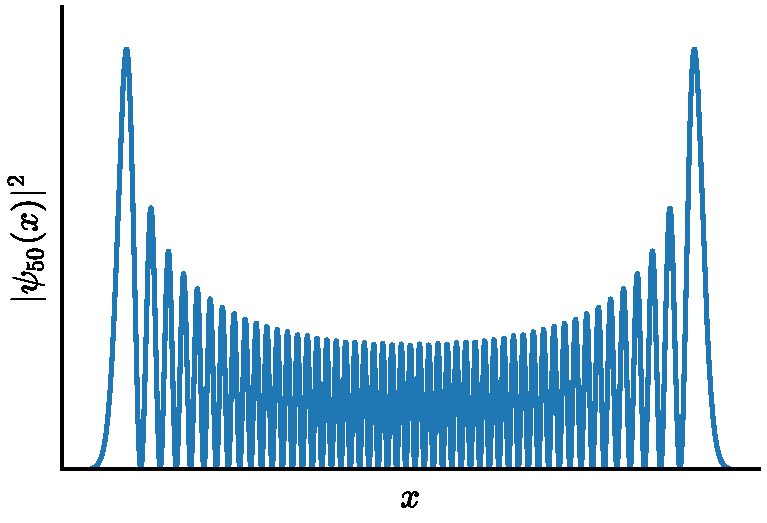
\includegraphics[width=0.5\linewidth]{hermite.pdf}
	\caption{The probability density function of the QHO with $n = 50$ contains nodes where the probability of finding the particle is zero. 
	The general profile also resembles the probability density of a classical harmonic oscillator.}
	\label{fig:qho-50}
\end{figure}

There are two interesting properties of this probability density function. 
First, notice that there are nodes where the probability of finding the particle is zero, just like the particle in a box. 
This is true of all energy states above the ground state. 
Second, we notice that the profile looks very different from the ground state; namely, the regions of largest probability are at the sides instead of the middle. 
This actually corresponds to a classical harmonic oscillator if you think about it---a moving mass on a spring with high elastic potential energy will spend the longest amount of time when it's most stretched out or most compressed (it moves the slowest as it changes direction), whereas it will move the fastest when it passes the equilibrium position (so the probability of finding it there is low, assuming it vibrates continuously without loss). 
Thus we see a nice analogy where the high-energy quantum mechanical system begins to exhibit classical behavior.


% % % % % % % % % % % % % % % % % % % % % % % % % % % % % % % % % % % % % 
% % % % % % % % % % % % % % % % % % % % % % % % % % % % % % % % % % % % % 
% % % % % % % % % % % % % % % % % % % % % % % % % % % % % % % % % % % % %
\section{Summary}

Whew! This was a lengthy chapter that was heavy on operators and bra-ket notation. 
Using ladder operators, we derived the ground state of the quantum harmonic oscillator, from which one can theoretically construct all the stationary states. 
We also discovered zero-point energy and determined that the allowed energies of the QHO are evenly spaced by $\hbar\omega$. 
I hope you found the derivations conducive towards your learning, and please come talk to me in office hours if something is unclear! 
Students find it helpful to try deriving some of these equations on their own to ensure full understanding. 
In the next chapter we will explore quantum field theory as an extension of the concepts presented here.

%} % for doublespacing
%\end{document}